\chapter{Technology Review}
This chapter will focus on the technical aspects of the projects by reviewing the technologies that make up the final version of the applied project. It will outline the reason these technologies were chosen, what the advantages and disadvantages of using these technologies was and the role of these technologies within the system.

\section{Overview} \\
For this project it was determined that a full stack development would be preferred, with this in mind it was important to determine what technologies would be suitable for a project such as this and which of these technologies would be most compatible with one another. Prior to taking on this project, the author had had experience using the MEAN stack in one previous module, the MEAN stack is an acronym for the use of the technologies MongoDB, Express, Angular and NodeJs. As previously mentioned, the author wished to use this project to both learn of new technologies and to polish up on some previously exercised technologies. For this purpose the stack used in the development of this project was as follows: \\
\begin{itemize}
    \item Angular for front end purposes (Previous experience)
    \item NodeJs for server-side purposes (Previous experience)
    \item Firebase for authentication purposes (New Technology)
    \item Firebase for database purposes (New Technology)
    \item Heroku for application deployment (New Technology)
\end{itemize}

\section{Core Technologies} \\
This section will discuss the core technologies that were implemented in the development of the web application. \\ \\

\subsection{Angular} \\
Angular is a typescript based, web-application framework, used to develop single-page web-applications. A single-page web-application is one which has all of the functionality of a multi-paged web-application but without the need to refresh the browser whenever the page of the web-application has been changed. Other frameworks that can be used to create single-paged web-applications are React, Django and Ionic. The popularity of single-page web-application has continued to grow in recent years. This rise in popularity can be linked back to the free flowing feeling these applications provide to the user rather than the stop-start mechanisms of a multi-page based web-application \cite{spa}

\begin{figure}[h!]
	\caption{The Architecture of Single-Page Application}
	\centering
	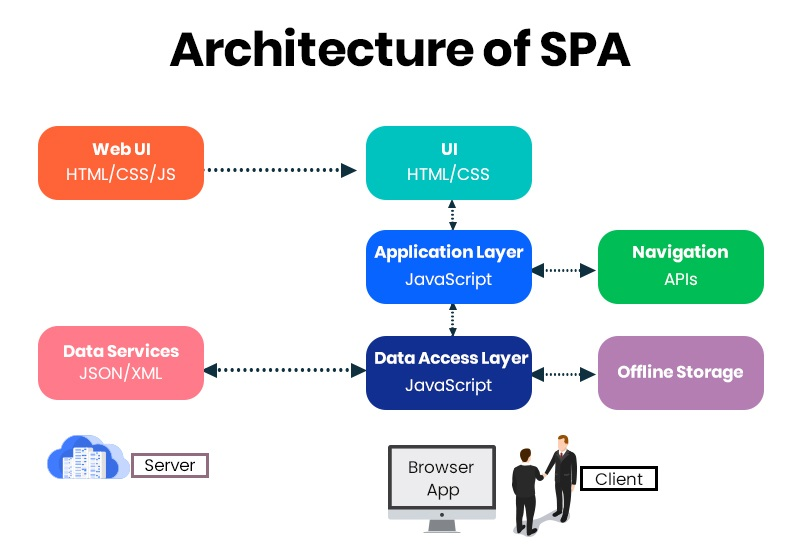
\includegraphics[width=0.9\textwidth]{images/spa}
\end{figure}

Angular was first released on October 20th 2010, as AngularJs, before experiencing a complete re-write and becoming the entity that we currently know it as today. As of the time of the writing of this paper Angular is currently on version 9, which was released on February the 6th 2020 and continues to grow the framework while fixing bugs \cite{angular}. \\ \\
For the purpose of this function Angular was chosen by the author because of the authors previous experience with it and being able to quickly discern that it was a reliable framework that was cooperative with other components. The author felt that improving on previous learning of the framework through independent learning would be beneficial as although the previous experience had been useful it resolved around MEAN stack implementation only whereas this proposed project would move away from that approach. \\
\begin{figure}[h!]
	\caption{Example of a typical HTML page in an Angular component}
	\centering
	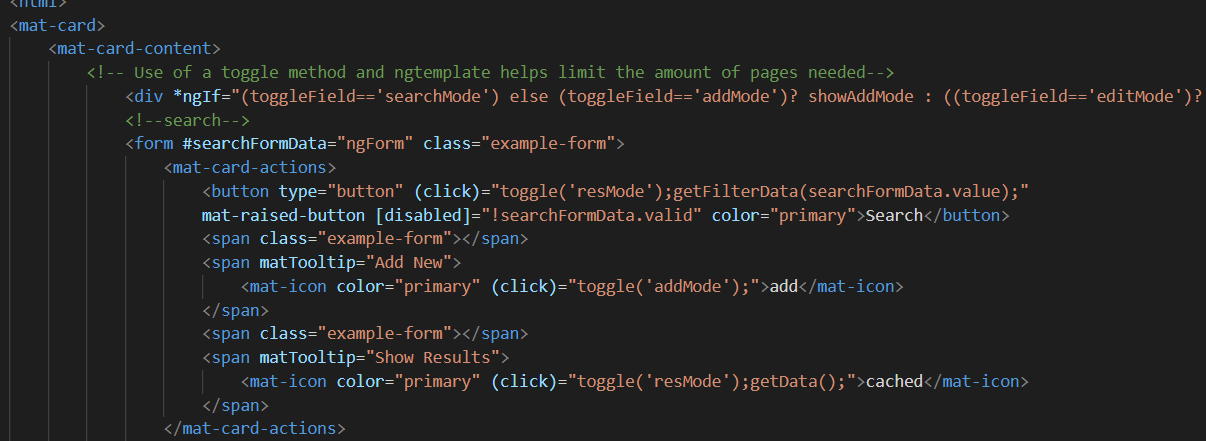
\includegraphics[width=0.9\textwidth]{images/angularhtml.png}
\end{figure}

\begin{figure}[h!]
	\caption{Example of a typical typescript page in an Angular component}
	\centering
	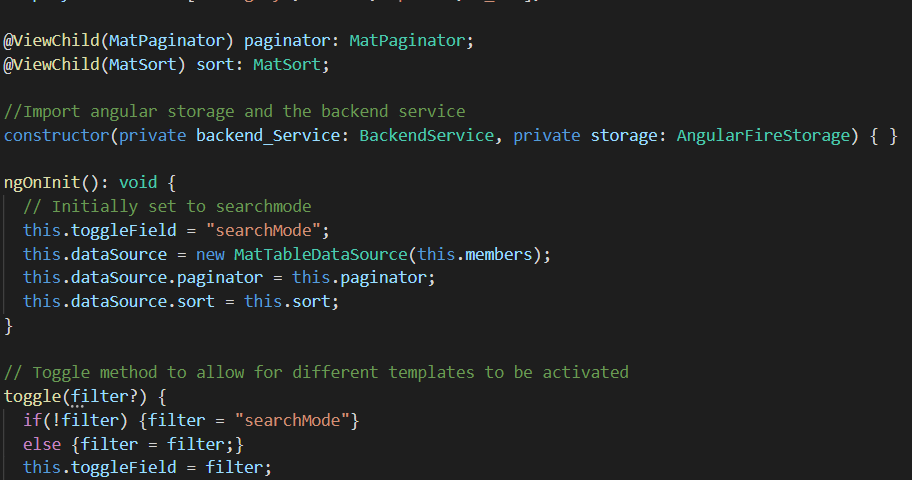
\includegraphics[width=0.9\textwidth]{images/angularts.png}
\end{figure}

\subsubsection{Angular-CLI}
Angular-CLI is a command line tool that used to aid in the development of an Angular based project. Through the Angular-CLI the application can be built and served and new services can be easily generated.

\subsubsection{Typescript}
Typescript is a superset of the programming language Javascript.It is compiled as javascript, which essentially makes it javascript plus additional features. Developers with experience of javascript will easily be able to adapt to using typescript when developing a web-application.  

\begin{figure}[h!]
	\caption{Example of a function written in typescript}
	\centering
	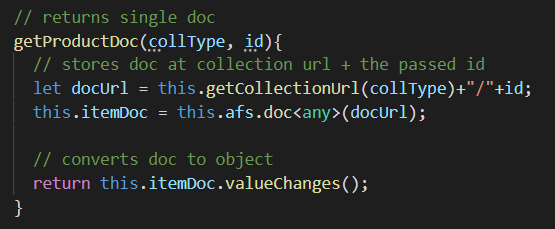
\includegraphics[width=0.9\textwidth]{images/tscode.png}
\end{figure}

\subsubsection{HTML}
HTML stands for Hyper Text Markup Language. HTML constitutes the "view" that the user of a web-application has. It is used to provide structure to the web-page and the features it creates on the web-page are provided functionality by the javascript/typescript. 

\subsubsection{CSS}
CSS stands for Cascading Style Sheets. CSS plays no role in the functionality of the web-application. The purpose of CSS is to make the web-application look appealing to users which is done by promoting a consistent styling throughout the entire web-application.

There are both advantages and disadvantages to using Angular framework: \cite{advdis} \\

\subsubsection{Advantages of Angular} \\
\begin{itemize}
    \item Model-View-Controller architecture of Angular allows the logic side of the application to be separate from the UI side of the application. Thanks to this architecture, problems within an Angular application can be more easily isolated.
    \item Custom directives, Angular allows for custom directives such as ngModel, which provides two way data binding to HTML form elements, directives such as these allow for improved HTML functionality and for  improved and more dynamic client-side applications.
\end{itemize} \\

\subsubsection{Disadvantages of Angular}  \\
\begin{itemize}
    \item Lack of CLI documentation. Developers have continually expressed concern over the lack of information in Angulars CLI documentation. Though the command line is highly usable within an angular project, a developer is likely to have to source information on potential commands from non-official sources.
    \item Steep Learning Curve. Many developers who are familiar with javascript and have branched into javascript based frameworks have made note of the fact that Angular, compared to other frameworks such as ReactJs, features a much steeper learning curve. This steep learning curve is due to the vast of array of topics and aspects of the framework that can be covered.
\end{itemize}

\subsection{NodeJs} \\
NodeJs is a cross-platform javascript run-time environment that allows for javascript to run outside of a browser. NodeJs features built in HTTP functionality, this allows a developer to utilize this HTTP functionality in a local environment wherein usually this would not be possible \cite{nodejs}. In the case of this project NodeJs is used for server-side purposes, meaning that the server-side and the front-end of the project both function using javascript which allows for a minimization of needed maintenance of the components of the project. \\ 
The reason NodeJs was used as a par of this project was that the author had previous experience with the technology and because of it's known compatibility with the Angular framework. Due to this easily maintained relationship with Angular, this offered more time to be attributed to exploring the new technologies being introduced to the author. Although the author has previous working experience with NodeJs, the environment on this occasion did not have NodeJs working in conjunction with Express as had been previously done. \\

\subsubsection{Node Modules} \\ 
NodeJs allows developers to make use of extra packages called Node Modules or NPMs. These packages usually provide extra functionality to an application, these packages provide a range of different functionality such as streamlined server connection and user authentication \cite{npm}. Throughout the development of this project NPM was used for providing server side connection to firebase and for the control of Angular modules and materials.

\begin{figure}[h!]
    	\caption{Popular NPM packages}
	\centering
	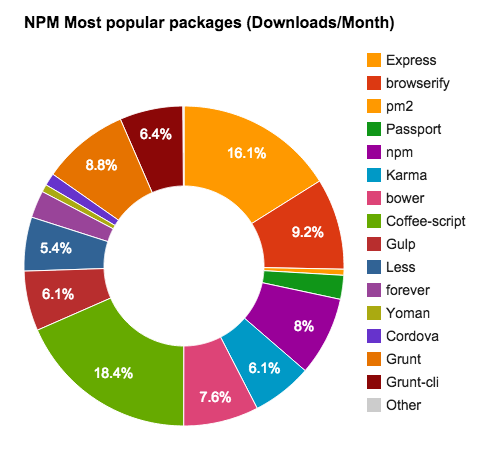
\includegraphics[width=0.9\textwidth]{images/npm.png}
\end{figure}

There are both advantages and disadvantages to using NodeJs\cite{advdis2}: \\

\subsubsection{Javascript}
Javascript is a programming language responsible for the functionality of web-pages. The javascript of a web-page allows for communication with the sever side of the application. In the case of this project, and many Angular based projects, typescript is used, which is a subset of javascript.

\subsubsection{Advatanges of NodeJs}
\begin{itemize}
    \item Easily Scalable. NodeJs can be used to scale an application either vertically or horizontally if needed. Single nodes within the server can make use of different resources which is not always available on javascript servers.
    \item Single Programming Language. Javascript is currently renowned as the most popular programming language in the world, as such, the fact that NodeJs can be completely run in javascript makes it a highly accessible server. The single use of javascript also makes NodeJs highly compatible with most web-application frameworks as the front-end functionality of these application is most commonly written using javascript as these applications are built to run on web browsers and most web browsers support javascript.
\end{itemize}

\subsubsection{Disadvantages of NodeJs}
\begin{itemize}
    \item Unstable API. The API of NodeJs is consistently changing and with this consistent change is a lack of stability. These new API changes often do not offer backwards compatibility and as such will require regular maintenance to occur if the application is to be stable and retain all functionality that was intended.
    \item Library Support. Compared to other programming languages such as Python and its flask server, javascript lacks a robust library system. This means that in some cases like in some parsing operations that NodeJs will have to rely on common libraries to complete these operations. As such it can go without saying that because NodeJs is reliant on javascript it actually adopts all of the weaknesses of javascript.
\end{itemize}

\subsection{Firebase} 
Within this project Firebase was used as both a database and for user authentication. Firebase is a Backend-as-a-Service (BaaS) created in 2011 before later being acquired by Google and being developed into a cloud platform. In the case of database use Firebase is largely similar to other document based databases such as MongoDB, this allowed for the learning curve to be easily navigated with any prior experience of working with document based databases to be of great help. However unlike traditional databases, Firebase removes the need for a back end server as would be usually expected on some stack development such as on the MEAN stack. Client SDKs allow for direct interaction to back end services which eliminates the need for middle-ware in these applications \cite{firebase}. \\
\begin{figure}[h!]
    	\caption{Traditional Infrastructure Vs Firebase}
	\centering
	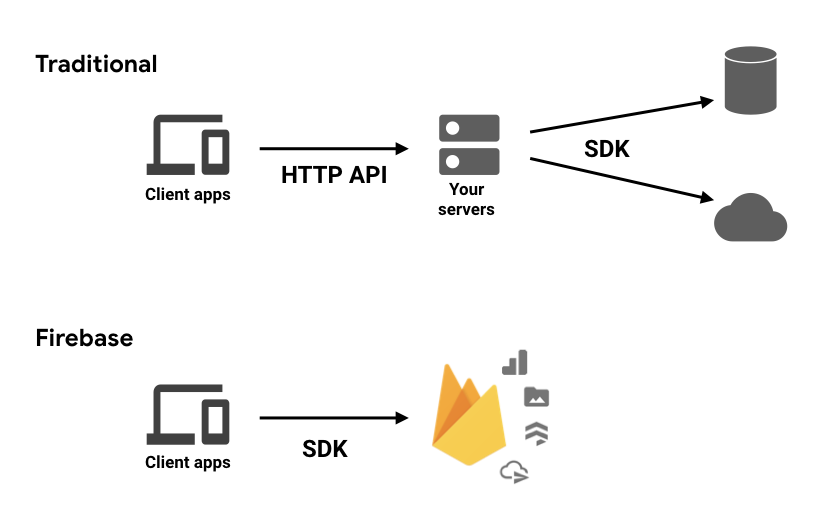
\includegraphics[width=0.9\textwidth]{images/firebase.png}
\end{figure}

\paragraph{}
Firebase was also used for user authentication purposes throughout the project. Firebase provides many SDKs and back end services that allow for user verification in a multitude of ways. Users can opt for sign in through social platforms such as Facebook or Twitter, standard E-mail and Password registration or through a Google(G-mail) account. In the case of this project the author has utilized the Google and E-mail/Password authentication \cite{fireauth}. When a user has been authenticated they will be granted an access token which will be attached to a unique id and either their email or the id of their social platform \\

\begin{figure}[h!]
    	\caption{How Firebase Authentication Works}
	\centering
	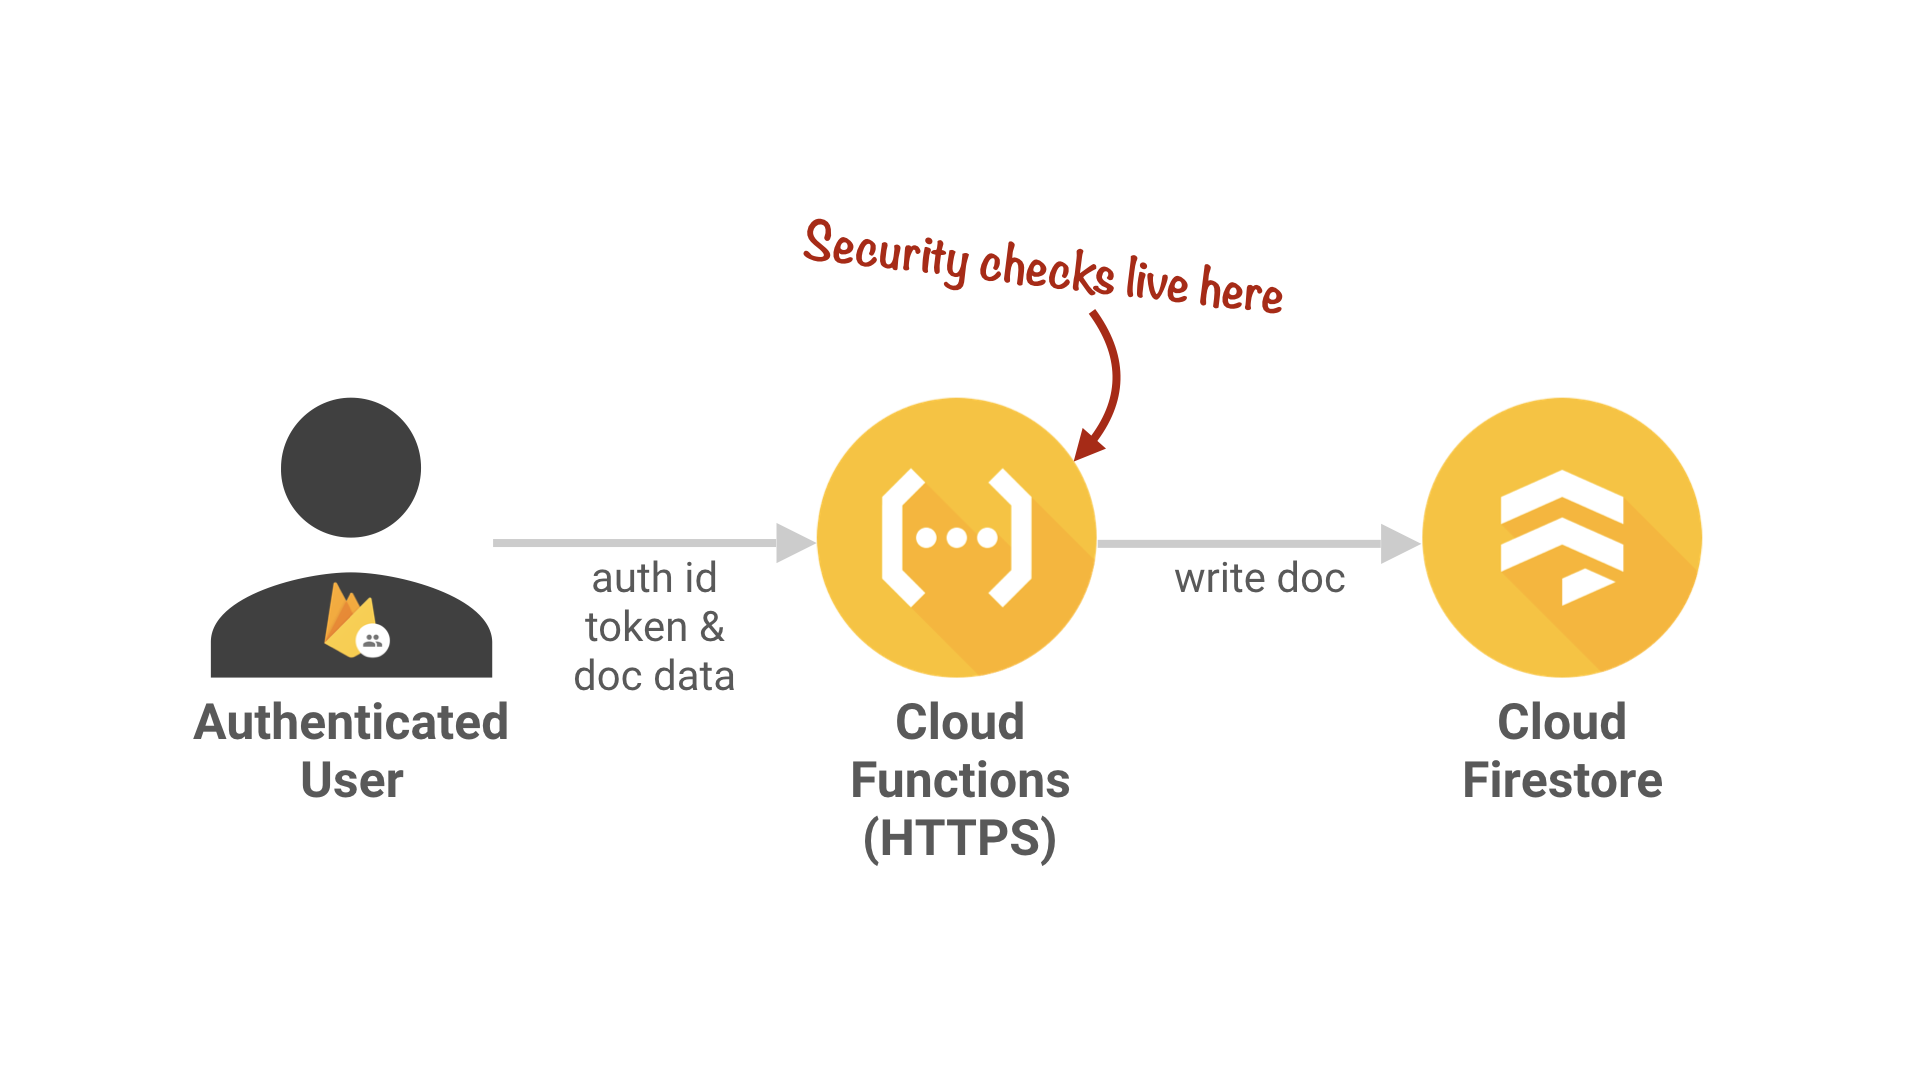
\includegraphics[width=0.9\textwidth]{images/fireauth.png}
\end{figure}
\\

\paragraph{}
Firebase also provides a variety of other products such as hosting of applications, however in the case of this project the author opted to use a different new technology for deployment and hosting of the web-application as it was determined by the author that it would be better for the project scope to explore new technologies and not become to reliant on a single technology when it was not required to do so. 

\subsubsection{Security}
Although a portion of the security related to Firebase was outlined when discussing Firebase user authentication, Firebase provides additional security in its database environment. Within Firebase the developer of a web-application using the database service can establish a set of "rules" to determine which users, if any, can access, read, write, edit or delete data. 
\begin{figure}[h!]
    	\caption{Example of a set of Rules in a Firebase database}
	\centering
	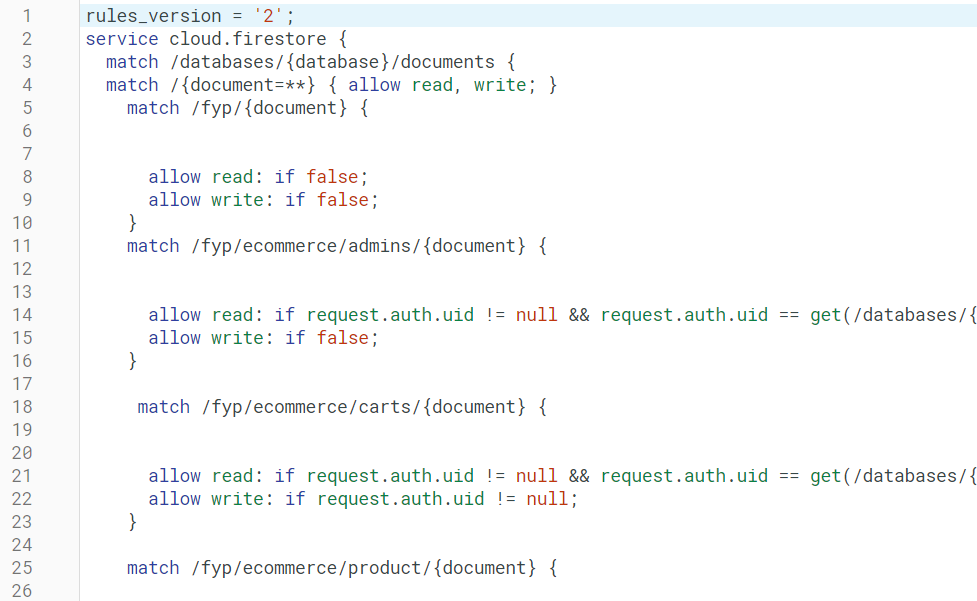
\includegraphics[width=0.9\textwidth]{images/fbrules.png}
\end{figure}

\subsubsection{JSON}
JSON, or Javascript-Object-Notation, is a lightweight format for storing and transporting data. JSON is text-based, making it readable by both human and machine. JSON is used by Firebase to store data for a number of reasons, it is easy for humans to read and write, it is language independent meaning it can be accessed by a number of programming languages and it supports many different data types\cite{inproceedings}. 

\begin{figure}[h!]
    	\caption{Example of JSON within a Firebase Database}
	\centering
	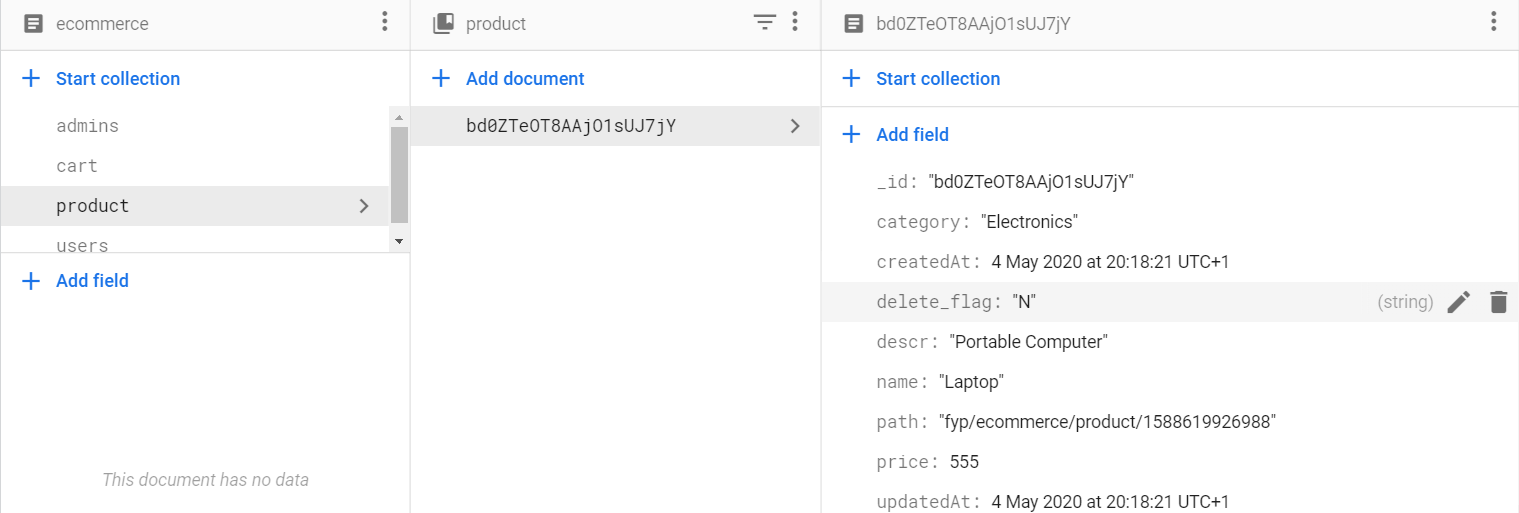
\includegraphics[width=0.9\textwidth]{images/jsonfb.png}
\end{figure} 
\newpage
There are Advantages and Disadvantages to using Firebase\cite{advdis3}: \\

\subsubsection{Advantages of Firebase}\\
\begin{itemize}
    \item Free start. Firebase provides a free starting point for all users, this means that until a certain data amount is reached or a specific service is required the use of Firebase is free to the user. 
    \item Documentation. Firebase provides users with extensive, detailed documentation on the methods, SDKs and the API. This allows for a low-barrier of entry for those who are new to Firebase as the documentation makes it easy to adapt to.
\end{itemize}

\subsubsection{Disadvantages of Firebase}
\begin{itemize}
    \item iOS Support. As Firebase is developed and maintained by Google, it is aimed more at working in conjunction with Android based applications. There are available supports to allow for iOS integration, however in that case it is easier to change to one of Firebases' competitors such as MongoDB.
    \item Database Limitations. Due to being entirely in JSON, the real time database used by Firebase is limited to simple read, write, update and delete queries. 
\end{itemize}

\subsection{Bootstrap}
Bootstrap is a library of css files available as open-source. Bootstrap is used to aid in the development of the UI of a web-application. Bootstrap is imported as part of the main css file available in every Angular project. As part of the authors project bootstrap is used in collaboration with Angular Materials to create the header file present throughout the entire web-application.

\subsection{Angular Materials}
Angular Materials are a series of optional modules that can be imported, developed by Google. The purpose of these modules is similar to that of bootstrap in that they are mainly for an aesthetic purpose. Throughout the project Angular Materials are used on many elements such as buttons, forms and icons. Angular Materials were used with Bootstrap on some features. 

\subsection{LaTeX}
LaTeX is a markup language similar to HTML. The use of LaTeX to construct this paper was a requirement of the course work. LaTeX uses tags to indicate what should happen to the write up when it is compiled. This LaTeX document was constructed and compiled using Overleaf.com. After it has been compiled to a text document, Overleaf allows for the document to be exported as a PDF. 

\begin{figure}[h!]
    	\caption{Example of Overleaf side by side source code with text document output}
	\centering
	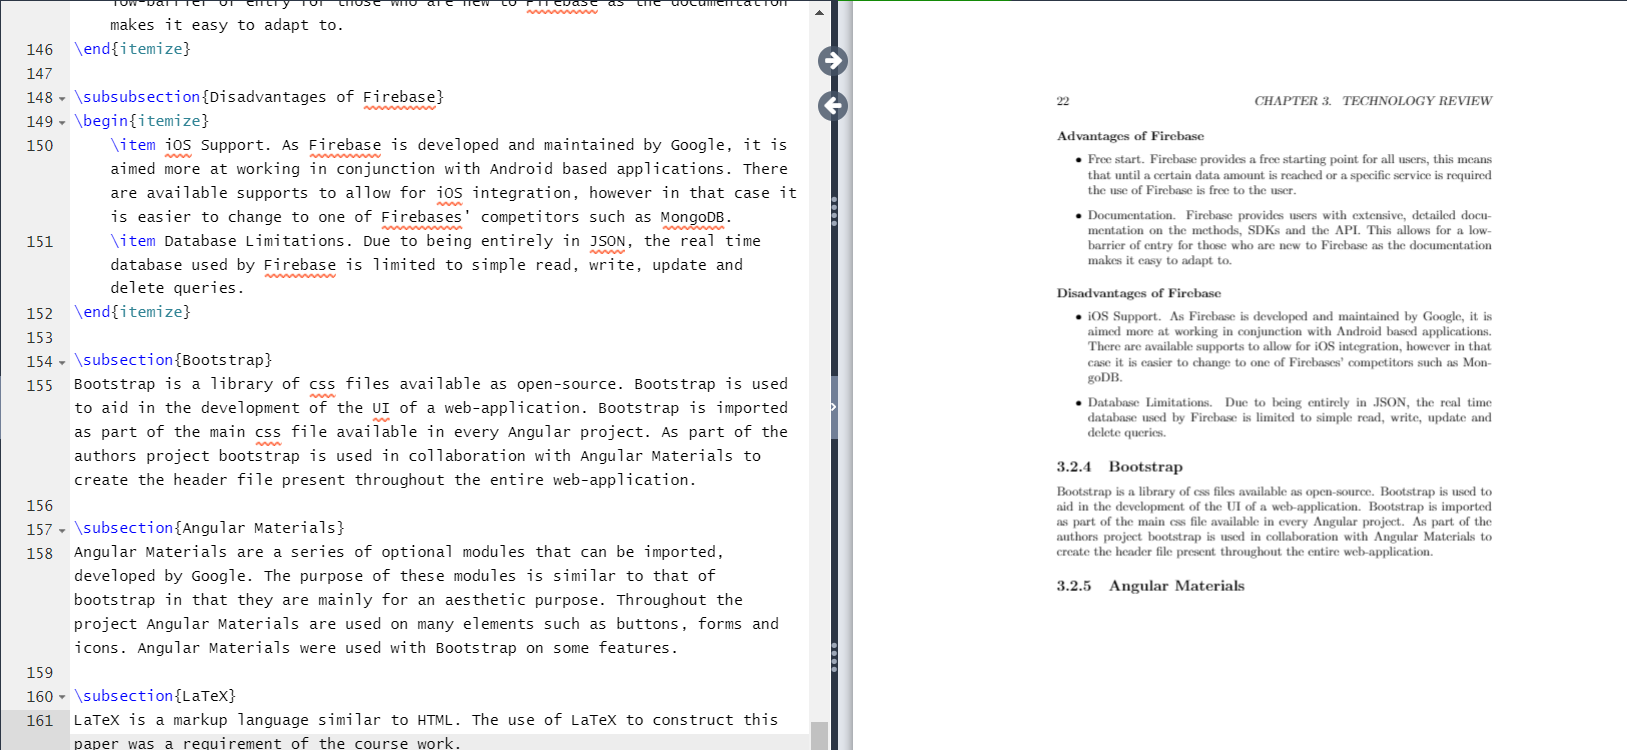
\includegraphics[width=0.9\textwidth]{images/overleaf.png}
\end{figure}

\begin{figure}[h!]
    	\caption{Example of this subsection in latex language before compilation}
	\centering
	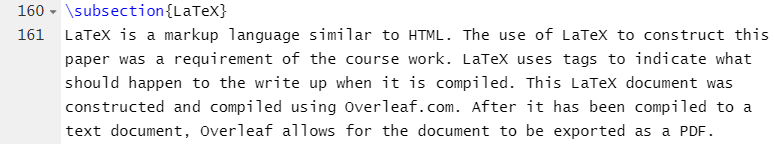
\includegraphics[width=0.9\textwidth]{images/latex.png}
\end{figure}

\subsection{Heroku}
Heroku is a Platform as a Service (PaaS), used for the deployment of web-applications to a cloud platform. To perform this deployment all that is needed is a Heroku account and a Github profile. When pushed Heroku a URL is produced that allows universal access to the application. Heroku allows for the deployment of almost any type of application and for those that are not supported build packages are available to make the application deployable. 









